\documentclass{article} % For LaTeX2e
\usepackage{iclr2027_conference,times}

\usepackage[utf8]{inputenc}
\usepackage[T1]{fontenc}
\usepackage{hyperref}
\usepackage{url}
\usepackage{xurl}
\usepackage{graphicx}
\usepackage{booktabs}
\usepackage{multirow}
\usepackage{amsmath,amssymb}
\usepackage{xcolor}
\usepackage{enumitem}
\usepackage{CJKutf8}
\usepackage{paracol}
\usepackage[capitalise,nameinlink]{cleveref}
\crefname{figure}{Figure}{Figures}
\Crefname{figure}{Figure}{Figures}
\crefname{table}{Table}{Tables}
\Crefname{table}{Table}{Tables}

\newcommand{\bench}{\textsc{jy-crpg-bench}}
\newcommand{\game}[1]{\begin{CJK}{UTF8}{bsmi}#1\end{CJK}}
% A page holding only a float starts at the top, not centred.
\makeatletter\setlength{\@fptop}{0pt}\makeatother

% Anonymous ICLR submission: \iclrfinalcopy is off, so the style prints the
% review running head and the anonymous author block. For the camera-ready,
% restore \iclrfinalcopy and the author block.
% \iclrfinalcopy

\title{\raggedright\bench{}: A Long-Horizon Benchmark \\ for Frontier Models in an Open-World RPG}

\author{}

\begin{document}

\maketitle
% Figure 1 is placed in the introduction and belongs at the top of page 2;
% this keeps the title page free of top floats.
\suppressfloats[t]

%% Everything numeric in this paper is generated from the run data. Nothing is
%% typed. See figures/emit_numbers.py and check_consistency.py.
% generated by figures/numbers.py from catalog_snapshot.json and start.state
% regenerate before editing any number in the paper
% catalogue entries in the snapshot
\newcommand{\NsessionsTotal}{24}
% sessions at the default budget that played
\newcommand{\Nsessions}{19}
% model sessions
\newcommand{\Nmodels}{17}
% random-baseline sessions
\newcommand{\NrandomRuns}{2}
% vendors in the field
\newcommand{\Nvendors}{6}
% distinct agent labels
\newcommand{\Nlabels}{17}
% distinct agent labels among the scored sessions
\newcommand{\NlabelsPlay}{14}
% distinct model labels among the scored sessions
\newcommand{\NmodelLabels}{13}
% sessions that never sent a key
\newcommand{\Nnever}{2}
% sessions at another playtime
\newcommand{\NotherBudget}{1}
% service probes, excluded
\newcommand{\Nprobes}{2}
% default playtime, seconds
\newcommand{\Nbudget}{1200}
% default playtime, minutes
\newcommand{\NbudgetMin}{20}
\newcommand{\EactsTotal}{3240}
\newcommand{\EactsModels}{1810}
\newcommand{\EactsRandom}{1430}
\newcommand{\EactsMedian}{98}
\newcommand{\EactsMin}{26}
\newcommand{\EactsMax}{720}
% pooled actions per second
\newcommand{\Eaps}{0.152}
% screen reads by model sessions
\newcommand{\Ereads}{1490}
% key events submitted
\newcommand{\EkeysTotal}{6215}
% distinct keys submitted
\newcommand{\EkeysDistinct}{15}
% share on the four isometric axes
\newcommand{\EshareDiag}{0.735}
% share on the arrow keys
\newcommand{\EshareArrow}{0.050}
\newcommand{\EkeysEnter}{850}
\newcommand{\EkeysSpace}{175}
\newcommand{\Qbest}{0.898}
\newcommand{\QbestLow}{0.822}
\newcommand{\QbestHigh}{0.944}
\newcommand{\QbestN}{98}
\newcommand{\QbestLabel}{Codex CLI / GPT-5.6-sol / Pi}
\newcommand{\Qworst}{0.068}
\newcommand{\QworstLow}{0.046}
\newcommand{\QworstHigh}{0.100}
\newcommand{\QworstN}{337}
\newcommand{\QworstLabel}{Gemini 3.7 Flash}
% minutes before its first key
\newcommand{\QworstStart}{3.7}
% screen reads per hundred actions of the lowest-ratio run
\newcommand{\QworstReads}{99}
\newcommand{\Qrandom}{0.403}
\newcommand{\QrandomLow}{0.378}
\newcommand{\QrandomHigh}{0.429}
\newcommand{\QrandomN}{1430}
\newcommand{\QrandomKeys}{13}
% model sessions under the random floor
\newcommand{\NbelowFloor}{1}
\newcommand{\QunderVsRandom}{0.169}
% how many times below the random floor the lowest run sits
\newcommand{\QunderTimes}{5.9}
% median inter-action gap of the random baseline, seconds
\newcommand{\QrandomGap}{1.4}
\newcommand{\QslowA}{Qwen 3.8 Flash}
\newcommand{\QslowB}{Claude Sonnet 5}
% the shorter of their median think times, seconds
\newcommand{\QslowGap}{21}
% the larger of their action counts
\newcommand{\QslowActs}{51}
% sessions whose character record was read
\newcommand{\Sread}{11}
\newcommand{\Sunread}{8}
\newcommand{\Slevel}{1}
% experience accumulated by every run
\newcommand{\SexpSum}{0}
\newcommand{\Sskills}{1}
\newcommand{\SexpAny}{0}
\newcommand{\SlevelTwo}{0}
% sessions whose screen latched the world-map signature
\newcommand{\Smap}{8}
% scored sessions with no world-map contact of any kind
\newcommand{\Sstayed}{11}
% ratio of the steady-traversal run
\newcommand{\Qsteady}{0.748}
% its oscillation rate
\newcommand{\QsteadyOsc}{0.006}
% its action count
\newcommand{\QsteadyN}{159}
% its label
\newcommand{\QsteadyLabel}{Claude Fable 5}
% of those, corroborated by a black frame
\newcommand{\SmapFade}{4}
\newcommand{\SmapSolo}{4}
\newcommand{\SmapUnread}{10}
% minutes
\newcommand{\SexitMedian}{7.8}
\newcommand{\SexitFirst}{4.9}
\newcommand{\SexitLast}{10.4}
% median keys before a crossing
\newcommand{\SexitActs}{40}
% vendor families with a corroborated crossing
\newcommand{\SexitVendors}{2}
% character records addressed
\newcommand{\Mrecords}{320}
\newcommand{\MrecordBytes}{182}
% bytes of that block
\newcommand{\Mblock}{58240}
% records carrying a name
\newcommand{\Mnamed}{320}
% records exceeding hp/maxHp or mp/maxMp
\newcommand{\Moverflow}{2}
% key names the API accepts
\newcommand{\MkeyNames}{130}
% distinct scancodes behind them
\newcommand{\MkeyCodes}{100}
% --- derived strings used by the results table -------------------------
% each row: agent & second & first & keys & screen-changing decisions/n & ratio\ci{n} & in-going & map & end
% rows below are sorted by vendor then actions
% Claude Fable 5-1                 n= 209 k= 136 ratio=0.651[0.584,0.712] map=True level=1 exp=0 ttfa=11.15 reason=time
% Claude Fable 5                   n= 159 k= 119 ratio=0.748[0.676,0.809] map=None level=None exp=None ttfa=18.55 reason=time
% Claude Fable 5-1                 n= 123 k=  67 ratio=0.545[0.457,0.630] map=True level=1 exp=0 ttfa=22.93 reason=time
% Claude Opus 5                    n= 114 k=  96 ratio=0.842[0.764,0.898] map=None level=None exp=None ttfa=18.88 reason=time
% Vista / Claude Opus 5            n=  75 k=  51 ratio=0.680[0.568,0.775] map=True level=1 exp=0 ttfa=10.66 reason=time
% Claude Fable 5-1                 n=  66 k=  48 ratio=0.727[0.610,0.820] map=True level=1 exp=0 ttfa=18.38 reason=time
% Claude Sonnet 5                  n=  51 k=  42 ratio=0.824[0.697,0.904] map=None level=None exp=None ttfa=11.65 reason=time
% Gemini 3.7 Flash                 n= 337 k=  23 ratio=0.068[0.046,0.100] map=None level=None exp=None ttfa=219.5 reason=time
% Gemini 3.7 Flash                 n=  86 k=  66 ratio=0.767[0.668,0.844] map=None level=1 exp=0 ttfa=9.63 reason=time
% GLM-5.3 Flash                    n= 104 k=  82 ratio=0.788[0.700,0.856] map=None level=1 exp=0 ttfa=40.33 reason=time
% GLM-5.3 Flash                    n=  77 k=  56 ratio=0.727[0.619,0.814] map=True level=1 exp=0 ttfa=32.96 reason=time
% Codex CLI / GPT-5.6-sol / Pi     n=  98 k=  88 ratio=0.898[0.822,0.944] map=True level=1 exp=0 ttfa=12.51 reason=time
% GPT-5.6-sol                      n=  70 k=  55 ratio=0.786[0.676,0.866] map=True level=1 exp=0 ttfa=47.08 reason=time
% Vista / Codex / GPT-5.6-sol      n=  26 k=  23 ratio=0.885[0.710,0.960] map=False level=1 exp=0 ttfa=12.8 reason=idle
% Grok 4.6                         n= 116 k=  76 ratio=0.655[0.565,0.735] map=None level=None exp=None ttfa=18.52 reason=time
% Qwen 3.8 Flash                   n=  51 k=  29 ratio=0.569[0.433,0.695] map=True level=1 exp=0 ttfa=57.79 reason=time
% Qwen 3.8 27B NVFP4               n=  48 k=  41 ratio=0.854[0.728,0.928] map=None level=None exp=None ttfa=17.65 reason=time
% Random Baseline                  n= 720 k= 290 ratio=0.403[0.368,0.439] map=None level=None exp=None ttfa=0.48 reason=time
% Random Baseline                  n= 710 k= 287 ratio=0.404[0.369,0.441] map=None level=None exp=None ttfa=0.52 reason=time
% --- repetition of a label appears in the catalogue ----------------------------
% repeated GLM-5.3 Flash: [0.7272727272727273, 0.7884615384615384] spread=0.061
% repeated Claude Fable 5-1: [0.5447154471544715, 0.7272727272727273, 0.6507177033492823] spread=0.183
% repeated Gemini 3.7 Flash: [0.7674418604651163, 0.06824925816023739] spread=0.699
% repeated Random Baseline: [0.4027777777777778, 0.4042253521126761] spread=0.001

\input{tables/books.tex}

\begin{abstract}
A long-horizon task requires a model to perceive its environment, decide for
itself what is worth doing, and hold one plan across hours of dependent
decisions. We present \bench{}, which places a frontier model inside Heroes of Jin Yong, a 1996 open-world role-playing game whose ending requires the fourteen books of the Jin Yong novels. The model plays it as a person does, from the screen and the keyboard alone, which requires reading $320\times200$ isometric pixel art and 16-pixel Traditional Chinese and knowing the novels its world is built from. It has no quest log, marker or score, so the model must keep its own map and goals, and it must win turn-based battles against the game AI. Progress is scored by milestones of the game itself and by completion time. Under a
\NbudgetMin{}-minute budget, in which a human speedrun finishes the game, the best of \NmodelsDistinct{} frontier models reaches \Ltop{} of the \Lrungs{} milestones in the only session that wins a battle, and no session holds a book. The models stall at four points: leaving the first area, finding the entrances on the world map, acting on instructions given in dialogue, and winning the first battle. Two of these act as filters that a session passes early or not at all, and four-hour sessions of \NlongModels{} models get no further, while experienced human players hold a book within \LhumanBookLast{} minutes.
\end{abstract}

\section{Introduction}
\label{sec:intro}

Frontier models solve competition mathematics and write working compilers
\citep{deepmind2025imo,carlini2026compiler}, yet the tasks they complete reliably are still measured in hours of human
work \citep{kwa2025horizon}. A long horizon is a property of the task, the
number of dependent steps its completion requires \citep{chen2026horizongap},
and several of the benchmarks that measure it are text environments, business
simulations \citep{backlund2025vending,fan2026ecommerce} or interactive
fiction \citep{phan2025textquests}. A game adds a requirement they leave
out: the model has to recover its own state from raw perception, because
nothing in the environment reports it. The game benchmarks that keep perception each relax another part of the problem: BALROG adds a text rendering of the state \citep{paglieri2025balrog}, ARC-AGI-3 removes language \citep{arc2026arcagi3}, and MineExplorer hands the model its objectives \citep{ju2026mineexplorer}. None pairs the screen and keyboard of a human player with a script other than English, as \cref{tab:related} shows.

\begin{figure}[!htb]
\centering
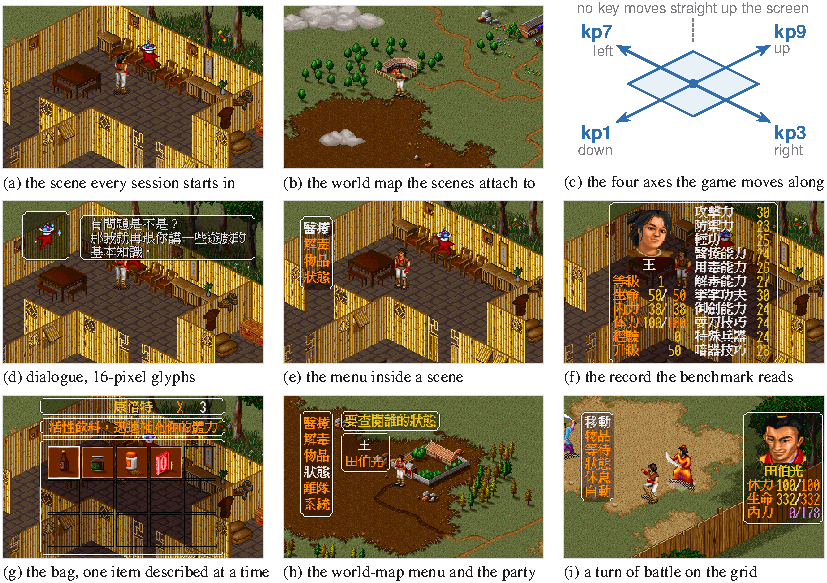
\includegraphics[width=\linewidth]{figures/env.pdf}
\caption{The game as a state chart of three states, each repeating the steps it lists, with the transitions between them. Every frame is one the model receives, upscaled three times without interpolation, and points at the state it shows, or at the dashed outline when it holds in every state.}
\label{fig:env}
\end{figure}

We present \bench{}, built on Heroes of Jin Yong, a 1996 Chinese role-playing game that we run unmodified under emulation. Its ending requires recovering the fourteen books of the Jin Yong novels from an open world, and \cref{fig:env} shows how it is played. We chose the game because it tests five capabilities of a frontier model at once.
\begin{enumerate}[leftmargin=*,topsep=2pt,itemsep=1pt,parsep=0pt]
\item The model must read the screen. The frame is $320\times200$ pixel art in a $45^\circ$ isometric projection, and every objective, prompt and statistic on it is Traditional Chinese in 16-pixel glyphs, a script that multimodal evaluation has largely neglected \citep{tam2025vistw}. No text is supplied to the model.
\item The model must bring knowledge the game never states. The world is assembled from the fourteen novels, so who a character is, which faction to join and which storyline leads to a book are known to a reader of the novels and written nowhere on screen.
\item The model must set its own goals. The game keeps no quest log, draws no marker and reports no score, so the model maintains its own map and plan and decides for itself what is worth doing. ARC-AGI-3 places the same goal-setting requirement at the centre of agentic intelligence \citep{arc2026arcagi3}.
\item The model must act through a keyboard alone, exposed through an API that it calls as a tool. Movement runs along four diagonals, no key moves straight up the screen, and every system of the game is a menu.
\item The model must win battles. Battles are turn-based on a grid against the AI of the game, with position, range and internal energy to manage, and a party at level one can lose them.
\end{enumerate}
Together these form one long-horizon task, a persistent world with sparse and delayed reward over thousands of dependent steps. The benchmark gives the model only what a person playing the game has, the frame on screen and the keys of the keyboard, with no state interface, text rendering, high-level action or memory built for a model, so its difficulty is that of the game as a person plays it. \Cref{sec:related} reviews related benchmarks, \cref{sec:bench} describes the benchmark, and \cref{sec:results} reports the results.

\begin{table}[!htb]
\centering
\caption{Game benchmarks for language-model agents. Observation is what the model receives before any upscaling, action is what it sends, and the last column is the record that verifies progress.}
\label{tab:related}
\footnotesize
\setlength{\tabcolsep}{2pt}
\begin{tabular}{@{}llllll@{}}
\toprule
Benchmark & Environment & Observation & Action & Language & Progress from \\
\midrule
\textbf{\bench{}} & one 1996 CRPG & 320$\times$200 px & keys & Trad.\ Chinese & memory, save, replay \\
\midrule
BALROG & 6 research games & text, render & text & English & env.\ reward \\
TextQuests & interactive fiction & text & text & English & game state \\
ARC-AGI-3 & abstract puzzles & 64$\times$64 grid & 6 actions, click & none & env.\ score \\
VideoGameBench & 1990s action games & native px & keys, mouse & English & checkpoint images \\
GameWorld & 34 browser games & browser & mouse, keys, API & English & game state \\
MineExplorer & Minecraft & 3D render & skill calls & English & milestone rules \\
\bottomrule
\end{tabular}
\end{table}

\section{Related Work}
\label{sec:related}

\subsection{Long-Horizon Evaluation}

The benchmarks that measure long horizons differ in what they hand the model
and in what they isolate. Most report the state in text. Vending-Bench
established long-term coherence as the property that separates long-horizon
tasks from long chains of short ones \citep{backlund2025vending}, and
E-Commerce Bench extends the setting to a year of deterministic business
operation \citep{fan2026ecommerce}. Both keep perception out of the loop.
TextQuests poses open-ended play over a long horizon in interactive fiction,
without vision \citep{phan2025textquests}, and TextAtari stretches horizons to
$10^5$ steps over text renderings \citep{li2025textatari}. Others isolate one
part of the problem: ARC-AGI-3 isolates adaptation to novel tasks by excluding
language and external knowledge \citep{arc2026arcagi3}, AutumnBench probes
world-model quality through environment-level queries
\citep{warrier2025benchmarking}, and UltraHorizon makes exploration under
hidden rules the task itself \citep{luo2025ultrahorizon}. \citet{kapoor2026openworld}
observe that benchmark design has favoured tasks that are precisely
specified, automatically graded and short, and call for open-world
evaluation. \bench{} keeps the state on the screen and the language in the game, leaves the subgoals beyond the opening to the model, and scores the whole task by the progress it yields, so it locates where a session stops without isolating why. Navigation, where two of the stall points of \cref{sec:results} lie, is a documented weakness even without perception: one-shot maze navigation fails by ten cells a side for every model tested \citep{jiang2026lostaggregation}, and from coordinates alone the failures are attributed to looping \citep{einarsson2025mazeeval}. Long horizons also complicate measurement: the ABC checklist catalogues task-validity and outcome-validity failures across agentic benchmarks \citep{zhu2025establishing}, and an audit of agent traces finds reward hacking in a majority of them on two suites \citep{shao2026validity}.

\subsection{Game Environments as Agent Benchmarks}

Games have been the standard setting for sequential decision-making since the
Arcade Learning Environment \citep{bellemare2013arcade}, and language and
vision-language agents have produced a second generation of game benchmarks.
BALROG aggregates six reinforcement-learning environments under one protocol
and reports a persistent gap between what a model knows about a game and what
it does inside one \citep{paglieri2025balrog}. lmgame-Bench isolates how much
of a game result belongs to the harness \citep{hu2026lmgame}, and Orak spans
twelve popular titles with configurable agentic modules \citep{park2026orak}.
VideoGameBench is the nearest benchmark to ours, running real 1990s games from raw pixels under a no-scaffold rule \citep{zhang2025videogamebench}.
GameWorld
standardises the action interface across 34 browser games and pairs every
task with a state-verifiable metric \citep{ouyang2026gameworld}. MineExplorer
evaluates open-world exploration in Minecraft and finds that models handle
single-hop tasks but degrade once hidden prerequisites must be coordinated
over a longer trajectory \citep{ju2026mineexplorer}.

The nearest precedents in horizon are the public Pok\'emon runs. Claude 3.7 Sonnet reached three
gym badges from screen pixels with a memory scaffold, where an earlier
model had not left the first house \citep{anthropic2025pokemon}. Gemini 2.5
Pro finished Pok\'emon Blue with a harness that translated the
RAM of the game into text \citep{comanici2025gemini}. The PokeAgent Challenge turned the setting
into a speedrunning track scored by completion time over milestones
\citep{karten2026pokeagent}. PokeGym builds a long-horizon benchmark on the
open-world game Pok\'emon Legends: Z-A with no access to game state
\citep{zhang2026pokegym}, and StarBench one on the turn-based Honkai: Star
Rail \citep{zhang2025starbench}. Crafter established the single-environment,
achievement-based design we follow \citep{hafner2021benchmarking}, and
NetHack remains the deepest environment in use for learned agents, with runs of tens of thousands of turns \citep{kuttler2020nethack}. Cradle and Voyager drive games through a foundation model with a skill library or a code API \citep{tan2024cradle,wang2023voyager}.

\section{Benchmark Design}
\label{sec:bench}

\subsection{Environment}
\label{sec:env}

Heroes of Jin Yong, published by Heluo Studio in 1996, is an open world of two tiers: one world map of $480\times480$ tiles \citep{scarsty2026kyscpp} and \Mscenes{} locations attached to it, such as buildings, sects and caves. \Cref{fig:env} draws the game as three states. The player enters a location from the world map and exits back to it, and inside a location a story event or a challenge starts a battle. A battle is turn-based on a grid: each turn a character moves along the four axes and then strikes, uses an item, waits or rests, and skills draw on internal energy. A won battle returns to the location, and a lost one either ends the game or lets the story continue. The game states its goal only through its story: enter the world of the Jin Yong novels, join its factions, learn its martial arts, and recover the fourteen books that end the game. \Cref{app:glossary} gives the Chinese original of every name from the game.

The game fixes the order of its opening and leaves the campaign open. It starts in a small house with a fenced yard, a searchable chest, one speaking character and one exit tile, and beyond the exit the path south across the world map leads to the hermit. His house, the starting house and five inns are the \MscenesOpenStart{} locations open at the start. \Cref{fig:route} in \cref{app:infra} shows the route. A cabinet beside the hermit holds the compass, the only source of coordinates the game offers, and his conversation opens all but \MscenesClosedHermit{} of the other locations, among them the house of the first party member, who joins after a yes-or-no prompt. The opening ends there without a battle, and the order of play after it is left to the player. The campaign runs through battles, the experience and levels that victories bring, and the chains of items, factions and battles that lead to the books. With all fourteen books and enough reputation, the ending is a final battle \citep{bahamut2023walkthrough}.

\subsection{Observation and Action Space}
\label{sec:interface}

The model observes the raw framebuffer at $320\times200$ and acts by pressing
keys. A scored session serves the native frame without upscaling, annotation,
set-of-marks overlay or accessibility tree \citep[cf.][]{xie2024osworld}. The frame combines several documented weaknesses of vision-language models. Low resolution reduces their accuracy \citep{niu2025resolution}, and images far from the training distribution degrade recognition even of familiar categories \citep{lin2026oodbench}. Text rendered as pixels is understood less well than the same text supplied as
tokens \citep{liu2026vistabench}, and precise spatial reading fails once
primitives are small or adjacent
\citep{rahmanzadehgervi2024blind,wang2024spatialeval}. The action space is
the keyboard of \MkeyCodes{} keys, and \cref{fig:keymap} shows the few the game responds to. Movement runs along the four numpad diagonals, with the arrow
keys aliased onto the same axes, so a model that presses \texttt{up} expecting
to walk up the screen moves up and to the right.

The single action presses a key, or a list of up to \MmaxKeys{} keys in order, holding each for a requested number of emulated frames. It returns once the screen has settled, including after a change of location, so the frame the model receives is the one to act on. There is no call that advances the game without input. The model can save and load through the menu of the game but cannot restore snapshots of the emulator, and \cref{tab:api} lists the calls. \Cref{app:infra} states the settle rule in frames, and \cref{app:design} gives the reasons for the list action and for the other choices of the protocol.

\subsection{Harness and Session Protocol}
\label{sec:protocol}

The benchmark supplies the instructions and the control surface, and the model plays through an agent harness. The hour sessions ran inside pi\footnote{\url{https://github.com/badlogic/pi-mono}}, a minimal coding agent, installed without modification and set to its high thinking level. Its four tools read, write and edit files and run a shell, from which the model drives the control surface with HTTP calls. The model receives one prompt, which names the instructions and sets the rules of the session: it may not read other conversations, look up walkthroughs or code online, or restart, and it reads and writes files only in a folder of its own. The instructions cover the session call, the calls that constitute play, the opening route as far as the compass, and a manual of the controls and systems of the game. They are published as \texttt{agents.md} in Chinese, which every model in this paper reads, and in an English translation, and \cref{app:instructions} gives the prompt and the instructions in both languages side by side. An action returns only its metadata unless the model asks for the frame in the same reply, so the model looks at the screen when it decides to. The benchmark adds no memory scaffold, no map, no pathfinder and no access to the state of the game. A model keeps any memory between actions in files it writes in that folder, and a scored session receives no field that reports its progress until it ends, so a model cannot query its own score. A session that reads the catalogue or the timelines of other sessions does not count. The leaderboard ranks models under one fixed harness, since harness choice changes game results \citep{hu2026lmgame,karten2026harness} and on long-horizon tasks the variance a harness induces can exceed the variance between models \citep{zhang2026harness}.

A session is created with a declared model name and a playtime, and its
clock starts at the first playable moment. The budget is played time, as for the human references and as in ARC-AGI-3 and TextQuests \citep{arc2026arcagi3,phan2025textquests}. The game advances only on input, so, as on a chess clock, a model thinks as long as it likes before each action and the time counts against its budget. Token counts are not comparable across closed multimodal models, whose image encoders are not published. Each session is a separate emulator process with a private copy of the game and its save slots reset to a new game, so no session inherits the progress of another. A session ends when its budget lapses or the game is completed. It then renders its recording to a time-compressed
video, computes its metrics, and appends itself to the public catalogue with the video and its keypress timeline. \Cref{fig:apparatus} shows the apparatus, and \cref{app:infra} lists the emulation parameters.

\begin{figure}[!htb]
\centering
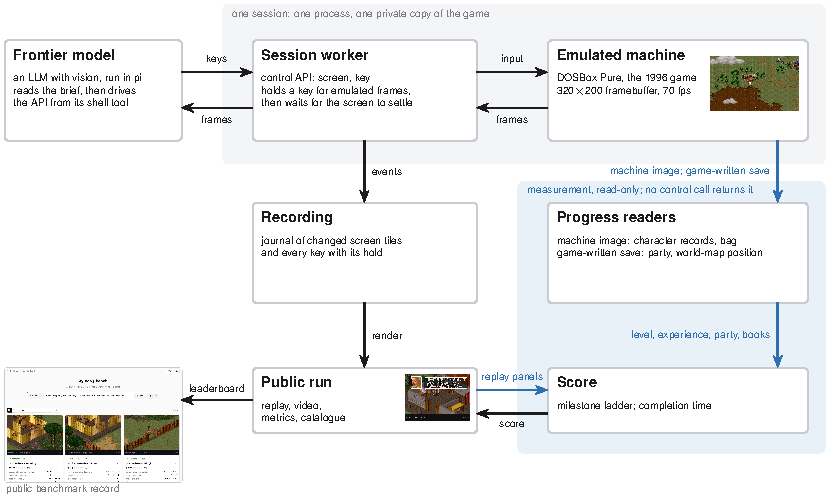
\includegraphics[width=\linewidth]{figures/architecture.pdf}
\caption{A frontier model in pi plays through the control API of its own session. Blue marks the measurement, which reads the memory of the emulator, the saves of the game and the on-screen events of the replay, and which the model cannot see.}
\label{fig:apparatus}
\end{figure}

\subsection{Progress Measurement}
\label{sec:measure}

Progress is read from records the model never sees: the state of the game, in the memory of the emulated machine and in the saves the game writes, and the published replay. The state gives the inventory, the compass, the books, the party and the level and experience of the leader. The game keeps seven events only on screen: the model enters a location from the world map, speaks with the hermit, opens the item screen with the compass in it, enters a battle, loses it or wins it, or answers the prompt of a party member who asks to join. Each draws fixed art at a fixed screen position, so these events are read by matching every frame of the replay against that art. A milestone, once observed, stays credited, so an item picked up and later used still counts. \Cref{app:measure} lists the record behind each milestone and checks the readings against one another.

The milestone scale has \Lrungs{} steps, following the achievements of Crafter \citep{hafner2021benchmarking}: six in the opening and five in the campaign. The opening milestones are the exit tile, the chest in the first room, a location entered from the world map, the conversation with the hermit, the compass in his cabinet, and the party member who joins through dialogue. The campaign milestones are a battle entered, a battle ended, won or lost, experience gained, the second level, and the first of the fourteen books. The milestones are listed in the order of the opening route, with the optional chest after the exit, and a session is credited with every milestone it reaches, so the count does not depend on the path taken.

The milestones extend to the ending of the game. The fourteen books are required before the final battle, and the saves record every book held, so the count of books continues the scale beyond the last milestone. The ending, read from the replay, gives the completion time that ranks the sessions that finish.

\section{Evaluation}
\label{sec:results}

We evaluate \NmodelsDistinct{} models from \Nvendors{} vendors at the
\NbudgetMin{}-minute budget, which is sized to the opening, with \NsessionsPlayed{} sessions on record and \LsessionsMin{} to
\LsessionsMax{} per model. A model is credited with every milestone any of its
sessions reached\ifnum\Naliased>0{}, and a session created under a variant of a model name, a spelling or the thinking level, is listed under the model\fi. The service ends a session after ten minutes without an action, which stopped \NidleSessions{} of the \NsessionsPlayed{} sessions before the hour. The baseline is a random policy that plays the same budget through the same control surface without reading the screen \citep{mnih2015humanlevel,hafner2021benchmarking,arc2026arcagi3}. Its \NrandomRuns{} sessions replay one key sequence drawn from seed \QrandomSeed{}, and \cref{app:design} gives the distribution of its keys. The human references are read from published videos of the game, \NhumanSpeedruns{} speedruns and \NhumanPlaythroughs{} playthroughs by experienced players, scored by the milestone readings of a replay, which \cref{app:measure} describes.

\subsection{Main Results}

Of the \Lmodels{} models, \ifnum\Lmap=\Lmodels all \Lmap{}\else\Lmap{}\fi{} reach the world map, \Litem{} pick up an item, \Lhermit{} speak with the hermit, and two take the compass, enter a battle and see it end. \LtopLabel{} reaches \Ltop{} of the \Lrungs{} milestones in one of its \LtopSessions{} sessions, which recruits a party member and wins a battle whose experience lifts the hero to the second level, and \LsecondLabel{} reaches \Lsecond{} across its \LsecondSessions{} sessions. No session holds a book. \Cref{fig:ladder} shows, for each model, the share of sessions that reached each milestone, with the human references in its two top rows. The speedruns, all of which finish the game in \LhumanSpeedCompletionMin{} to \LhumanSpeedCompletionMax{} minutes, cross onto the world map within the first minute in \LhumanSpeedStepsMin{} to \LhumanSpeedStepsMax{} keypresses and hold the first book between minutes \LhumanSpeedBookFirst{} and \LhumanSpeedBookLast{}. The playthroughs, one of which reaches the ending, hold it between minutes \LhumanPlayBookFirst{} and \LhumanPlayBookLast{}.

\begin{figure}[!htb]
\centering
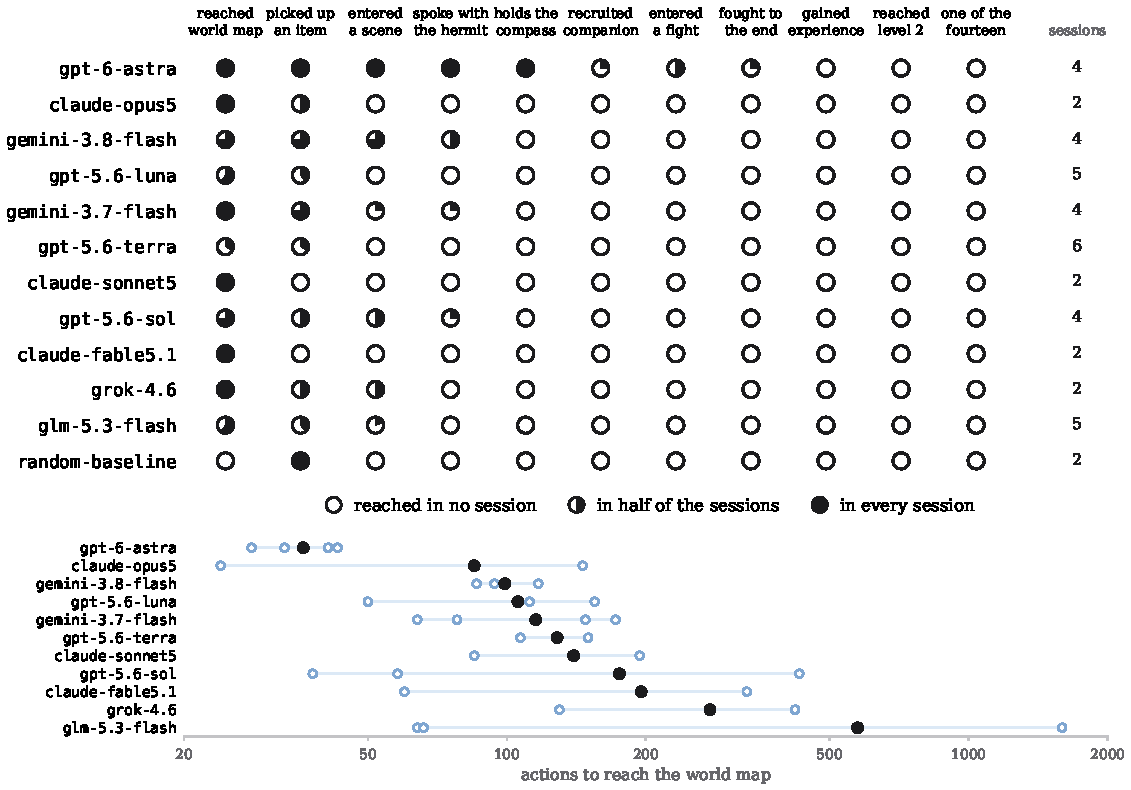
\includegraphics[width=\linewidth]{figures/ladder.pdf}
\caption{Milestones per model. The rows of the upper panel are ordered by the milestones reached and the rows of the lower panel by the mean keypresses to the world map, with the random baseline last. In the upper panel each marker shows the share of sessions in which the model reached the milestone, with the number of sessions at the right. The lower panel shows the keypresses to the world map across the sessions that crossed, on a log scale, with a light dot per session and a black dot for their mean. The two human rows are read from published videos, and \cref{app:measure} gives the record behind each milestone.}
\label{fig:ladder}
\end{figure}

\subsection{Behavioural Analysis}

The random policy reaches \QrandomRungs{} of the \Lrungs{} milestones in \QrandomBudgetMin{} minutes, since a random walk in a small room reaches the chest within the hour. The world map is the first milestone a random walk does not reach. The chest therefore separates models from one another but not from the baseline: \Litem{} models searched it and \LnoItem{} never did. Beyond the chest the models stall at four points, and \cref{fig:frames} in \cref{app:measure} shows frames from each.

\begin{figure}[!htb]
\centering
\includegraphics[width=0.86\linewidth]{figures/routes-compound.pdf}
\caption{The walk of every model through the starting house in its session with the most milestones, from the spawn tile (circle) to the crossing (square). The colour gives the minute of play on the scale of \cref{fig:world} and the arrowheads the direction. The panels follow the upper panel of \cref{fig:ladder}, and \cref{app:measure} describes how a walk is read.}
\label{fig:compound}
\end{figure}

The first is the gate of the starting house, where the model must map its keys onto the isometric view. The yard is closed by a fence with one gate, and \cref{fig:compound} draws the walk of every model through it. Every model crosses onto the world map, in \LcrossSessions{} of the \NsessionsPlayed{} sessions, and \LcrossEvery{} models cross in every session they played, but the gate is found by trial. The median crossing took \SexitActs{} keypresses, and \PexitActsMaxLabel{} pressed \PexitActsMax{} keys in one session, walking into the fence until minute \PexitMinMax{}. The count varies more within a model than between models, as the lower panel of \cref{fig:ladder} shows: the crossings of \LspreadLabel{} differ by a factor of \LspreadRatio{} and the means of the models by a factor of \LbetweenRatio{}.

The second is finding the entrances on the world map, the same problem at a larger scale, since the entrance of a walled house is one tile on one face. After the crossing the rest of the hour is spent on the world map, and \cref{fig:world} draws three walks on it. \Lscene{} models entered a location from it, for all but \LtopLabel{} and \LsecondLabel{} an inn or the house of the hermit, and the other \LnoScene{} stayed on the world map or went back into the starting house. \PorbitLabel{} crossed at minute \PorbitExitMin{}, then spent \PorbitActs{} actions and \PorbitMin{} minutes on the world map without entering a location, passing the gate of the hermit repeatedly.

\begin{figure}[!htb]
\centering
\includegraphics[width=0.86\linewidth]{figures/routes-world.pdf}
\caption{Three walks on the world map in the first hour, coloured by the minute of play: the session of \LtopLabel{} with the most milestones, the session of \LsecondLabel{} that entered the most locations, and the session of \PorbitLabel{} that stayed longest on the world map without entering a location. A numbered marker stands at the last point on the world map before a location entered or an event read from the replay, and the column at the right lists the markers with their minutes. A gap in a path is a visit to a location or a loaded save.}
\label{fig:world}
\end{figure}

The third is the dialogue of the hermit, where the model must turn what it reads into an action. The instructions name the cabinet beside him, and his conversation names it again. \Lhermit{} models reach the conversation, in \PhermitSessions{} sessions. \PtalkSlowLabel{} pressed through it for \PtalkSlowMin{} minutes and \PtalkFastLabel{} for \PtalkFastMin{}, and neither searched the cabinet. \LsecondLabel{} reached him in every one of its \LsecondSessions{} sessions, between minutes \PhermitEveryFirst{} and \PhermitEveryLast{}, and the \LhermitOthers{} other models that reached him did so in at most half of their sessions. The session of \PscenesMaxLabel{} in \cref{fig:world} searched the cabinet and used what it found, reading its coordinates from the compass \PholderMenuOpens{} times.

The fourth is the first battle, where the model has to recover from a defeat. All \PfightSessions{} sessions that entered a battle entered it in the house of Yan Ji. \LsecondLabel{} lost it at minute \PsecondDefeatMin{} in one session and sent its last key at minute \PbattleLastMin{} with it still open in another, and \LtopLabel{} lost it at minute \PtopDefeatMin{}. What separates the one win is what that session did next, as \cref{fig:recovery} shows: it recruited a party member at minute \PrecruitMin{}, returned to Yan Ji at minute \PreturnMin{} and won at minute \PwonMin{}, passing through all three states of \cref{fig:env}. No other session that lost a battle returned to it, and \cref{app:battles} compares the battles.

\begin{figure}[!htb]
\centering
\setlength{\tabcolsep}{1.5pt}
\begin{tabular}{@{}cccc@{}}
\includegraphics[width=0.24\linewidth]{figures/frames/battle/loss-4-defeat.png} &
\includegraphics[width=0.24\linewidth]{figures/frames/battle/win-1-party.png} &
\includegraphics[width=0.24\linewidth]{figures/frames/battle/win-3-energy.png} &
\includegraphics[width=0.24\linewidth]{figures/frames/battle/win-4-won.png} \\
\end{tabular}
\caption{The session of \LtopLabel{} that won a battle: the defeat of the hero alone, the party chosen on its return, an item that restores internal energy, and the battle won.}
\label{fig:recovery}
\end{figure}

\subsection{Four-Hour Sessions and Filters}
\label{sec:long}

A four-hour session counts when the service ended it at the budget with its last key in the final \NlongWindowMin{} minutes. Of the \NlongAttempts{} attempts, \NlongSessions{} by \NlongModels{} models count, and \cref{tab:long} lists them. \Cref{app:infra} gives the reasons the others do not, among them an attempt of \LlongHackLabel{} that broke the rule of its prompt by reading the timelines of earlier sessions.

\Cref{fig:filters} follows all \Nchain{} model sessions, hour and four-hour, through the steps a playthrough passes in order. Every step thins the population, and two act as filters: sessions pass them within the first \FilterWait{} minutes or not at all. Of the \NhermitRisk{} sessions that entered a location, \NhermitPass{} reached the hermit, all within \PhermitPassMax{} minutes, and none after \FilterWait{} minutes, although the others played \PhermitLateHours{} more hours beyond that point. Of the \NwinRisk{} that entered a battle, one won, within \FilterWait{} minutes, and none after, although the others played \PwinLateHours{} more hours. After their first hour the four-hour sessions pass no filter, and the one among them that lost a battle, of \LlongBeyondLabel{}, did not return to it in \PfThreeMin{} more minutes and \PfThreeActs{} actions.

\begin{figure}[!htb]
\centering
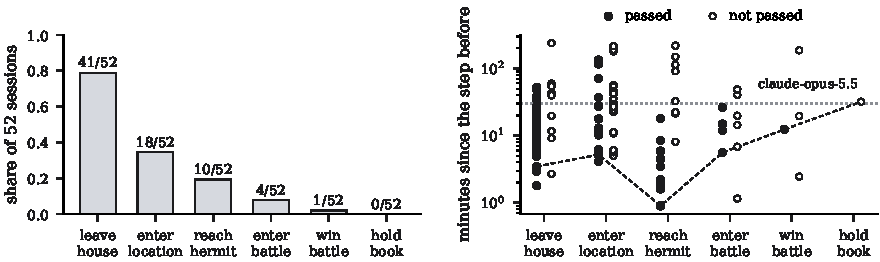
\includegraphics[width=\linewidth]{figures/filters.pdf}
\caption{All model sessions through the steps a playthrough passes in order. Left, the sessions that passed each step, of those that passed the step before. Right, for each of those, the minutes from the step before to passing it (filled) or to its last key (open); the dotted line marks \FilterWait{} minutes, and the dashed line traces the session of \LtopLabel{} that won a battle.}
\label{fig:filters}
\end{figure}

\section{Conclusion}
\label{sec:conclusion}

We presented \bench{}, a long-horizon benchmark in which a frontier model plays a 1996 open-world role-playing game with the screen and keyboard of a human player, scored by events of the game itself. Progress over this horizon is gated by filters. A session reaches the hermit or wins its first battle within its first \FilterWait{} minutes or never does, and neither more played time nor longer thinking changes that: the four-hour sessions pass no filter after their first hour, and the milestones a session reaches barely rise with the time its model thinks before each action. A stuck model spends the extra time repeating what it has tried: it walks into the same fence, circles the same gate or presses through the same dialogue. A long horizon thus measures which filters a model passes, and experienced human players pass all of them and hold a book within \LhumanBookLast{} minutes. Each filter asks for a capability of any general agent: grounding its actions in an unfamiliar view to find an entrance one tile wide, turning a line it reads into the action it names, and revising its plan from the outcome of its own actions. The one session that won a battle did the last: it lost, recruited a party member and returned to win, although no instruction describes that plan. Since more time at test does not supply these capabilities, they have to come from training across many environments that demand them, including small text in scripts other than Latin. Longer sessions and a first-time human player under the same instructions will extend the scale into the campaign.

\subsection*{AI use statement}
We used generative AI tools, coding agents built on frontier language models, throughout this work. They implemented the benchmark service, the replay scanner and the scripts that generate every number, figure and table in this paper from the session records. They recovered and reformatted session records, supported the qualitative analysis of the replays, and proposed and refined parts of the measurement design. They searched for and formatted related work, and they drafted and edited the text of this paper under our direction. We have not used generative AI tools to generate synthetic data, to formulate or prove mathematical claims, or to propose hypotheses. The models evaluated in the benchmark are the object of study. We have reviewed all AI-assisted work. Every number in the paper is regenerated from the session records at each build, every typed claim about the records is verified by a consistency script, and the frames and readings behind the qualitative analysis were checked against the replays. We take responsibility for the final content of this work, including text, claims and artifacts produced with the aid of generative AI.

\subsection*{Ethics statement}
The benchmark runs a commercial 1996 game that is not redistributed: every host supplies its own copy, and the frames in this paper identify the interface under study, as \cref{app:licence} explains. The work involves no human participants, and the public catalogue carries the metrics, videos and keypress timelines of model sessions and no personal data.

\subsection*{Reproducibility statement}
The benchmark code, the instructions the models receive, the replay scanner and the scripts that generate every number, figure and table in this paper will be released with the paper, and an anonymised copy of the code base is in the supplementary material. \Cref{app:instructions} gives the instructions in full. The release includes the records, videos and keypress timelines of every session in this paper. \Cref{app:infra} lists the emulation parameters and the dates of the sessions, \cref{app:design} gives the reasons for the protocol choices, and \cref{app:measure} the readings behind every milestone. The game itself is not redistributable, as \cref{app:licence} states.

\bibliography{refs}
\bibliographystyle{iclr2027_conference}

\appendix
\crefalias{section}{appendix}
\crefname{appendix}{Appendix}{Appendices}
\Crefname{appendix}{Appendix}{Appendices}

\section{Release and Licensing}
\label{app:licence}
The benchmark service, its public submission system and the leaderboard are released on acceptance of this paper, and the supplementary material holds an anonymised copy of the code base for review. The benchmark code is released under MIT. The emulation core
(\texttt{dosbox\_pure\_libretro}) is GPLv2 and is loaded at runtime through the libretro C API. The bundled macOS core is built from \texttt{schellingb/dosbox-pure} at \texttt{7f6e8fb}, and the hosted
service ships a Linux build pinned by image digest. The game is the 1996
commercial release, copyright Soft-World International and
Heluo Studio. It is not redistributable or tracked in the repository, and every host supplies its own copy. The copy the paper was measured with is identified by two SHA-256 digests, one of the program file the launcher loads and one of a manifest over the 616 shipped files without the three rewritable save slots, with one line per file, sorted by name, giving digest and name.\\ \texttt{\footnotesize Z.DAT\quad 0034f836def2b287e62b0902f08cab22b61b397f24d44d6038274f1750a007ce}\\ \texttt{\footnotesize manifest\quad 29ef75ab32a7905e0b274a9bba9e9ea0ff1b081e74aeacedf86350604aedc558}\\ The public catalogue carries only the metrics, videos
and replay timelines we measured, and nothing that substitutes for the game
data. The frames of the game in this paper
identify the interface under study, as prior work showing frames of
copyrighted games has done \citep{paglieri2025balrog}.

\section{Interface and Session Details}
\label{app:infra}
\Cref{tab:api} lists the control surface, and \cref{fig:keymap} shows the keyboard the API exposes. Emulation is DOSBox Pure through libretro at a fixed 26800 cycles with no sound card, so the observation is visual only. The published video runs at \DefaultReplaySpeed{} times speed, or faster for long runs, with a strip naming the model, the action number, the keys held and the clock, beside a timeline file with every keypress and its hold.

Each key is held for a requested number of emulated frames, ten by default, because the game samples its keyboard once per loop. The action returns once the screen has settled: the game has \MsettleReact{} frames to react, and the wait then ends after \MsettleStable{} frames without change, when the picture cycles as in an idle animation, or after \MsettleMax{} frames regardless. A black frame marks a change of location, and the action waits through it and settles once more.

The hour sessions ran from \FieldDates{} and the four-hour sessions from \LongDates{}. \Cref{tab:effort} lists the effort of every model in the quantities the service records: sessions, actions, keys per action and the time between actions, and \cref{tab:milestones} gives each milestone in actions and in minutes, the medians over the sessions that reached it. The sessions took between \EactsMin{} and \EactsMax{} actions. Neither the time a model thinks between actions nor how often it looks set the order of the milestones reached: over the \NcadenceSessions{} model sessions, their rank correlation is $\CrhoThink$ with the median think time and $\CrhoKeys$ with the keys per action, and over the \NlookSessions{} sessions whose record counts the screen reads, where the median read the screen \ClookMedian{} times per action, it is $\CrhoReads$ with the reads per action. \PbatchLabel{} sent lists of up to \PbatchMaxKeys{} keys in one action, \PbatchKeysPerAction{} on average, so it looked at the screen once for every \PbatchKeysPerAction{} keys it pressed.

The catalogue also holds sessions the paper leaves out: \NexcludedSessions{} of \LexcludedLabel{}, a model with two later versions in this paper, and the \NlongWithheld{} four-hour attempts that do not count, of which \NlongZero{} sent no action, \NlongStartup{} sent one or two, \NlongEarly{} sent their last key before minute \NlongMinLastMin{}, \NlongExcluded{} were declared under names that identify no model of the paper, and one read the timelines of earlier sessions. That attempt, while stuck in the opening, fetched the keypress timelines of earlier sessions with its shell, read the key sequences of the fastest, and went on to hold the compass and recruit a party member. Reward hacking of this kind is common in agent traces \citep{shao2026validity}, and a long horizon gives a stuck model hours to look for it. The release lists each attempt with its reason.

\begin{table}[!htb]
\centering
\caption{The control surface. A check marks a call the model can use in a scored session; the snapshot calls serve development.}
\label{tab:api}
\footnotesize
\begin{tabular}{@{}llc@{}}
\toprule
Call & Meaning & Model can use \\
\midrule
\texttt{GET /api/screen} & the current frame & \checkmark \\
\texttt{GET /api/help} & the instructions & \checkmark \\
\texttt{GET /api/keys} & every accepted key name & \checkmark \\
\texttt{GET /api/slots} & emulator snapshots on disk & $\times$ \\
\texttt{POST /api/key \{"key":"kp3","hold":10\}} & press one key, or several in order & \checkmark \\
\texttt{POST /api/save \{"name":"..."\}} & take a snapshot & $\times$ \\
\texttt{POST /api/load \{"name":"..."\}} & restore a snapshot & $\times$ \\
\bottomrule
\end{tabular}
\end{table}

\begin{figure}[!htb]
\centering
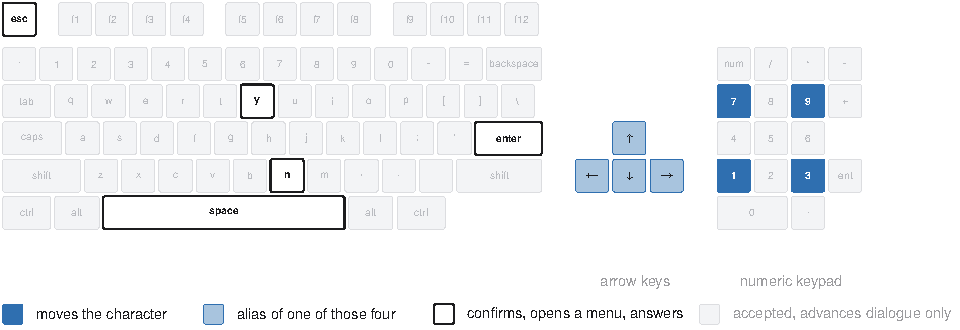
\includegraphics[width=0.8\linewidth]{figures/keymap.pdf}
\caption{The keyboard the API exposes, with the nine keys the game responds to outside dialogue highlighted; any key advances a dialogue.}
\label{fig:keymap}
\end{figure}

\begin{figure}[!htb]
\centering
\includegraphics[width=\linewidth]{figures/route-human.pdf}
\caption{The opening route as far as the hermit, from a human speedrun: (a) the starting house from the spawn tile to the gate, (b) the world map from the gate to the house of the hermit, and (c) that house from its door to the hermit. The walks are read and drawn as in \cref{fig:compound,fig:world}, coloured by the second of the speedrun; the house of the hermit is stitched from the frames of the speedrun.}
\label{fig:route}
\end{figure}

\begin{table}[!htb]
\centering
\caption{Effort per model in the order of the upper panel of \cref{fig:ladder}; actions and seconds are medians over sessions.}
\label{tab:effort}
\footnotesize
\renewcommand{\arraystretch}{0.86}
\input{tables/effort.tex}
\end{table}

\begin{table}[!htb]
\centering
\caption{Each milestone in actions and minutes: the sessions that reached it and the median action count and minute at which they did.}
\label{tab:milestones}
\footnotesize
% generated by figures/emit_milestones.py from the replays and timelines; do not hand-edit
\begin{tabular}{@{}lrrr@{}}
\toprule
Milestone & Sessions & Median actions & Median minute \\
\midrule
reached the world map & 32 & 86 & 16 \\
picked up an item & 22 & 20 & 3 \\
entered a location & 13 & 145 & 27 \\
spoke with the hermit & 9 & 101 & 19 \\
held the compass & 5 & 129 & 21 \\
recruited a party member & 2 & 270 & 37 \\
entered a battle & 3 & 158 & 27 \\
ended a battle & 2 & 172 & 22 \\
gained experience & 1 & 372 & 28 \\
reached level 2 & 1 & 372 & 28 \\
held a book & 0 & -- & -- \\
\bottomrule
\end{tabular}

\end{table}

\begin{table}[!htb]
\centering
\caption{The four-hour sessions that count, one row per session: the minute of the last key, the actions sent, the minute at which each milestone was first reached, and the milestones credited. The crossing is timed by the service and the other milestones by the replay; a dash marks a milestone not reached.}
\label{tab:long}
\footnotesize
\setlength{\tabcolsep}{1.5pt}
\resizebox{\linewidth}{!}{\input{tables/long.tex}}
\end{table}

\section{Design Decisions}
\label{app:design}

An action accepts one key or a list of up to \MmaxKeys{}, because a menu path or a repeated step is one decision. A list costs one round trip and one settle wait for the whole list. The coupling between perception and action is set by how often a model looks, since an action returns no picture unless asked, and a model that sends single keys without asking for the screen is as open-loop as one that sends twenty. The cap bounds the longest list, and every list is recorded in the public timeline.

The observation is the frame the game draws, at its own resolution, since reading sixteen-pixel glyphs and an isometric map is part of the task. The instructions list the on-screen terms in the Traditional Chinese the game draws.

The baseline is a seeded random policy because it measures what the milestone structure yields to chance: the small first room puts the chest within reach of a random walk, and no later milestone is. Each action draws one of the \QrandomKeys{} keys the instructions teach, the four diagonal movement keys with \QrandomMoveShare{} percent of the draws and the confirm key with \QrandomEnterShare{} percent, \QrandomPace{} seconds apart on average, until the budget lapses.


\section{Measurement Details}
\label{app:measure}

The world map is read from its frame; the item from the item message; the location from the name banner drawn on entry, the starting house excepted; the hermit from his portrait; the compass from the inventory or the item screen; the party member from the party size or a yes to the recruitment prompt; the battle from the card of the acting character; an ended battle from the defeat or battle-won message; experience and level from the character sheet in the save or the messages a won battle draws; and a book from the inventory or the items the hero carries.

% The frames are fixed evidence from this field, picked by hand from the
% published replays; the labels in the caption are the generated macros, so a
% regenerated field that changes who holds a pattern has to re-pick them.
\begin{figure}[!htb]
\centering
\setlength{\tabcolsep}{2pt}
\begin{tabular}{@{}ccc@{}}
\includegraphics[width=0.32\linewidth]{figures/frames/a-compass-read.png} &
\includegraphics[width=0.32\linewidth]{figures/frames/b-hermit-talk.png} &
\includegraphics[width=0.32\linewidth]{figures/frames/c-recruit-tian.png} \\
{\footnotesize (a) \LsecondLabel} & {\footnotesize (b) \LsecondLabel} & {\footnotesize (c) \LtopLabel} \\
\includegraphics[width=0.32\linewidth]{figures/frames/d-battle-won.png} &
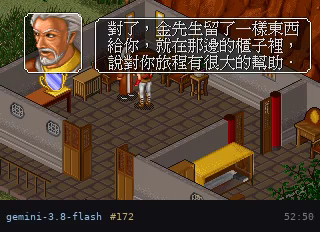
\includegraphics[width=0.32\linewidth]{figures/frames/e-cabinet-hint.png} &
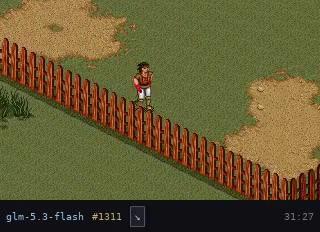
\includegraphics[width=0.32\linewidth]{figures/frames/f-fence-corner.png} \\
{\footnotesize (d) \LtopLabel} & {\footnotesize (e) \PtalkSlowLabel} & {\footnotesize (f) \PexitActsMaxLabel} \\
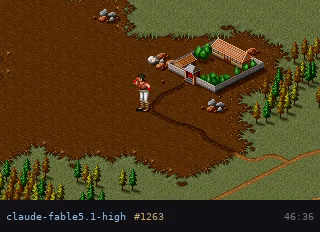
\includegraphics[width=0.32\linewidth]{figures/frames/g-gate-orbit.png} &
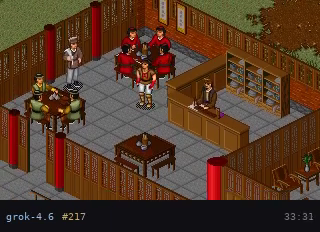
\includegraphics[width=0.32\linewidth]{figures/frames/h-inn-loop.png} &
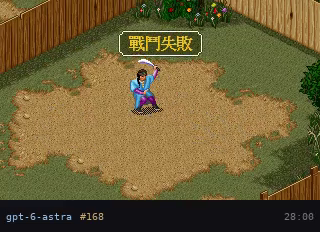
\includegraphics[width=0.32\linewidth]{figures/frames/i-defeat.png} \\
{\footnotesize (g) \PorbitLabel} & {\footnotesize (h) \texttt{grok-4.6}} & {\footnotesize (i) \LsecondLabel} \\
\end{tabular}
\caption{Frames from the replays behind the readings and the walks of \cref{sec:results}, each with the strip naming the model, the action count and the clock: (a) the compass coordinates on the item screen; (b) the conversation with the hermit; (c) the recruitment prompt of Tian Boguang; (d) the message of a battle won; (e) the hermit naming the cabinet; (f) the yard behind the fence; (g) passing the gate of the hermit; (h) talking to an innkeeper; (i) the defeat message.}
\label{fig:frames}
\end{figure}

Every replay frame is matched by normalised cross-correlation against nine templates, the fixed art of the on-screen events, and \cref{fig:frames} shows frames with them. A template counts when it scores above \ReplayThreshold{} for \ReplayHold{} seconds of play: two consecutive frames of a replay at \DefaultReplaySpeed{} times speed and one frame of a replay at 24 times. The game shows such art for a second or more, so a shorter match is a screen transition. Four messages are dismissed at the next key, so a single frame counts: the item message and the three that close a won battle, which announce the win, the experience gained and a new level. A recruitment prompt counts as a recruitment when the first key pressed after it appears is a yes. The walks of \cref{fig:compound,fig:world,fig:route} place every frame of a replay or video at the offset of highest normalised cross-correlation on a panorama of the starting house, stitched from the replays, or on the world map, rendered from the data files of the game. The world map scrolls to keep the hero at one screen position, which a compass reading of a replay fixes, so the offset of a frame gives his tile.

The human rows of \cref{fig:ladder} are read from \NhumanVideos{} published videos, \NhumanSpeedruns{} speedruns and \NhumanPlaythroughs{} playthroughs, listed in the release with the frame behind every reading. A capture is admitted when the first room of the starting house in a benchmark replay matches it at \HumanRoomGate{} or above, which locates the game frame and excludes the remakes of the game. The capture is scaled to the native frame and matched against the templates as a replay is, over a window of two pixels and at a threshold set per video in the gap of its score distribution. The clock starts where a benchmark session starts, on the first frame in which the hero stands on his spawn tile, and the crossing is the first black frame after it. An action is a tile step, read from the shift of the background on the lattice of the isometric tile, or a screen change without a step, such as a line of dialogue. A won battle and a level are read from the messages that announce experience gained and a new level, a book from the item message that names it, and the ending from the closing conversation with the hermit. A recruitment is read from the party list or from a battle in which a party member acts.

The readings agree wherever two records exist. Each of the \PobtainedBag{} sessions whose inventory shows a new item also shows the item message. The crossing count read from the replay agrees with the count the service recorded on all \LcrossAgree{} sessions that carry both. Of the \PcompassBoth{} sessions with both an inventory reading and a replay, every one of the \PcompassBag{} whose inventory holds the compass shows the coordinate line on the replay, and no other session does. Of the \PhermitBoth{} sessions with a preserved save and a replay, every one of the \PhermitOpened{} whose save shows the locations the hermit opens also shows his portrait on the replay. Where an event occurs, the five held templates score at least \ReplayHitMin{} and the four single-frame messages at least \ReplayMsgHitMin{}; elsewhere they score at most \ReplayMissMax{} and \ReplayMsgMissMax{}. The first reading of every template in the hour sessions, \NpanelAudited{} in all, was also checked by eye against its frame, and each shows the event.

\section{Battle Analysis}
\label{app:battles}
A battle is turn-based tactics on the grid of the location. The player chooses which party members fight, and on its turn a character moves along the four axes and then attacks with a martial art, uses poison, a cure, medicine or an item, waits, rests or hands the battle to the game. An attack draws on internal energy, so a character without it has no attack in its menu. \Cref{tab:battles} lists every battle on record, and \cref{fig:battles} sets the two battles of one session side by side.

All \Nbattles{} battles are fought against Yan Ji in the yard of his house. Of the \NbattlesAlone{} fought by the hero alone, \NbattlesAloneLost{} ended in defeat and one stayed open when the session stopped sending keys. The battle itself does not separate the win from the defeats: in the won battle \PwinConfirm{} percent of the keys confirmed the highlighted command, and the one step on the replay beyond confirming is an item that restores internal energy. What separates it is the plan around the battle. The session of \LtopLabel{} is the only one that returned to a battle it had lost, and it returned with a party member recruited in between. The \NlostNoReturn{} other sessions that lost a battle never fought again, one of them with \PnoReturnLeftMin{} minutes of its budget left. The sessions that recruited Duan Yu fought no battle afterwards.

\begin{table}[!htb]
\centering
\caption{Every battle on record, with the minutes it began and ended, and the actions and keys the model sent while it lasted, with the share of keys that confirm.}
\label{tab:battles}
\footnotesize
\resizebox{\linewidth}{!}{\input{tables/battles.tex}}
\end{table}

\begin{figure}[!htb]
\centering
\setlength{\tabcolsep}{1.5pt}
\begin{tabular}{@{}cccc@{}}
\includegraphics[width=0.24\linewidth]{figures/frames/battle/loss-1-party.png} &
\includegraphics[width=0.24\linewidth]{figures/frames/battle/loss-2-turn.png} &
\includegraphics[width=0.24\linewidth]{figures/frames/battle/loss-3-health.png} &
\includegraphics[width=0.24\linewidth]{figures/frames/battle/loss-4-defeat.png} \\
{\footnotesize (a)} & {\footnotesize (b)} & {\footnotesize (c)} & {\footnotesize (d)} \\
\includegraphics[width=0.24\linewidth]{figures/frames/battle/win-1-party.png} &
\includegraphics[width=0.24\linewidth]{figures/frames/battle/win-2-turn.png} &
\includegraphics[width=0.24\linewidth]{figures/frames/battle/win-3-energy.png} &
\includegraphics[width=0.24\linewidth]{figures/frames/battle/win-4-won.png} \\
{\footnotesize (e)} & {\footnotesize (f)} & {\footnotesize (g)} & {\footnotesize (h)} \\
\end{tabular}
\caption{The two battles of the session of \LtopLabel{} against Yan Ji. Lost, top: (a) the hero alone chosen to fight; (b) Yan Ji at full health; (c) the hero at low health; (d) the defeat message. Won, bottom: (e) the hero and Tian Boguang chosen; (f) Tian Boguang without internal energy and without an attack in his menu; (g) an item that raises internal energy; (h) the battle-won message.}
\label{fig:battles}
\end{figure}

\section{Prompt and Instructions}
\label{app:instructions}
The first row is the prompt each model is sent to start a session, and the rows after it are the instructions the prompt names. Every model in this paper reads the Chinese in the right column; the left column is its English translation, in the names of \cref{app:glossary}. In the prompt, \texttt{\{PLAYTIME\}} names the budget and \texttt{\{MODEL\_NAME\}} the model. The instructions are those of the 60-minute budget. Those of the four-hour budget differ only in the minutes value of the session call. The addresses of the site and of the hosted service are withheld as \texttt{SITE\_URL} and \texttt{SERVICE\_URL}.

\input{tables/instructions.tex}

\section{Glossary}
\label{app:glossary}
\Cref{tab:glossary} gives the Chinese original of every name from the game that the paper uses, and of the fourteen books, with the English titles of the novels they are named after.

\begin{table}[!htb]
\centering
\caption{Names from the game as the paper writes them and as the game writes them.}
\label{tab:glossary}
\footnotesize
\renewcommand{\arraystretch}{0.9}
\begin{tabular}{@{}l@{\hspace{2.2em}}l@{}}
\toprule
\begin{tabular}[t]{@{}ll@{}}
In the paper & In the game \\
\midrule
Heroes of Jin Yong & \game{金庸群俠傳} \\
Heluo Studio & \game{河洛工作室} \\
Soft-World International & \game{智冠科技} \\
the starting house & \game{王居}, \game{主角居} \\
the hermit & \game{南賢} \\
the house of the hermit & \game{南賢居} \\
inn & \game{客棧} \\
Heluo Inn & \game{河洛客棧} \\
Tian Boguang, his house & \game{田伯光}, \game{田伯光居} \\
Duan Yu & \game{段譽} \\
Yan Ji, his house & \game{閻基}, \game{閻基居} \\
Yaowang Manor & \game{藥王莊} \\
Fuwei Escort Agency & \game{福威鏢局} \\
Hengshan Sect & \game{衡山派} \\
Black Dragon Pool & \game{黑龍潭} \\
compass & \game{羅盤} \\
internal energy & \game{內力} \\
experience gained & \game{獲得經驗點數} \\
a new level & \game{升級了} \\
item message & \game{得到} \\
defeat message & \game{戰鬥失敗} \\
battle-won message & \game{戰鬥勝利} \\
\end{tabular} &
\begin{tabular}[t]{@{}ll@{}}
Book & In the game \\
\midrule
\booktable
\end{tabular} \\
\bottomrule
\end{tabular}
\end{table}

\end{document}
